% ============================================================================
% AD7031 Week 11-12 -- LECTURE NOTE, version WITH PROOFS (CVaR proposition, VaR <=> chance constraint)
% The classroom version OUU_week11_note.tex omits the two proofs.
%
% Straight conversion of the course folder's handwritten notes:
%   "OUU Lecture 3" p.2 (bottom) - p.4 : optimization under uncertainty, portfolio example,
%        stochastic optimization, risk measure, stochastic program, risk neutral, mean-variance
%   "OUU Lecture 4" p.1 - p.4 : Markowitz mean-variance as a convex QP, limits of
%        mean-variance (two pictures), VaR, CVaR, proposition CVaR = E[Z | Z >= VaR]
%        for continuous Z, proof via the derivative in beta
%   "OUU Lecture 5" p.1 - p.3 : proof finished (indicator, conditional expectation),
%        discrete example (atoms at -1, 0, 1; atom splitting), uncertainty in the
%        constraint: E / VaR / CVaR constraints, chance constraint, proposition
%        VaR constraint <=> chance constraint
% Robust optimization and DRO (Lecture 5 p.3 bottom - p.4) are not taught this year, so the
% "competing paradigms" overview and the shortest path example are gone.  Section 1 now sets the
% deterministic program and (SP) side by side; the portfolio example moved next to its figure.
% Section 2 takes uncertainty in the objective only (2.1-2.4 = the four risk measures), Section 3 in
% the constraints only, and Section 4 takes both.
% The first page recaps week 10 (chance constraint -> MIP) and is the only statement of it; the old 3.2 is gone.
% 2.4: the VaR / CVaR convexity trees follow the convexity quizzes the author pointed to; they use E, so
% they need no discreteness.  The discrete assumption is stated once, in 3.2, where a finite program needs it.
% Changes from the handwritten order: the hand-drawn "same P, different x, different
% loss" sketch (Lecture 3 p.3) is replaced by week09_loss_distribution.pdf, generated
% by loss_distribution_2d.py (two assets, Tech boom/bust vs quiet Energy, Gaussian
% regime mixture; the loss densities are exact 1-D mixtures).  Added at the end:
% the CVaR stochastic program with one beta per risk term, and its scenario LP
% (HW2 Problem 4(d)-(e)).
% Added after the VaR <=> chance constraint proposition: the chance constraint as a MIP, written
% through the violation form P(f > 0) <= eps so that z = 1 / z = 0 match the week 10 classification
% MILP (misclassified / correct).  Checked against brute-force scenario subsets (scipy/HiGHS).
% Added in 2.3-2.4: min_x VaR and min_x CVaR, the inner min joining the outer min over x.
% Section 3 reordered: the chance constraint and the VaR <=> chance proposition now come before the
% CVaR constraint, and each risk constraint shows its full problem with a deterministic f_0(x).
% Discrete example checked by hand: eps = 1/2, VaR = 0, CVaR = 1/2 (g(beta) = 1/2 + beta/2
% on [0,1], 1/2 - beta/2 on [-1,0]); E[Z | Z >= 0] = 1/3, E[Z | Z > 0] = 1, atom split 1/2.
% Same house style as OUU_week06_note.tex; self-contained -- no \input.
% ============================================================================
\documentclass[10pt]{article}

\usepackage[a4paper, margin=1.9cm]{geometry}
\usepackage{amsmath, amssymb, mathtools}
\usepackage[dvipsnames]{xcolor}
\usepackage{graphicx}
\usepackage{array}
\usepackage{colortbl}
\usepackage{tikz}
\usetikzlibrary{patterns}
\usepackage{dsfont}
\usepackage[hidelinks]{hyperref}

\definecolor{ruleink}{RGB}{18, 68, 140}
\definecolor{demoink}{RGB}{140, 82, 20}
\definecolor{keyink}{RGB}{20, 90, 20}
\definecolor{watchink}{RGB}{86, 60, 140}
\definecolor{punchink}{RGB}{170, 30, 60}
\definecolor{lineA}{RGB}{44, 110, 176}
\definecolor{lineB}{RGB}{168, 96, 32}
\definecolor{lineC}{RGB}{78, 62, 140}

% ---- the pens used in the handwritten original ----------------------------
\definecolor{redink}{RGB}{198, 38, 38}
\definecolor{purpink}{RGB}{132, 58, 176}
\definecolor{grnink}{RGB}{22, 118, 62}
\definecolor{magink}{RGB}{214, 30, 158}
\definecolor{boxink}{RGB}{232, 150, 42}
\definecolor{sandink}{RGB}{250, 206, 142}

\setlength{\parindent}{0pt}
\pagestyle{empty}

% tighter spacing around centered displays
\AtBeginDocument{%
  \abovedisplayskip=7pt plus 2pt
  \belowdisplayskip=7pt plus 2pt
  \abovedisplayshortskip=4pt
  \belowdisplayshortskip=4pt}

% ---- one section -----------------------------------------------------------
\newcommand{\beat}[2]{%   number, title
  \par\bigskip\vspace{4pt}
  {\color{ruleink}\rule{\textwidth}{1pt}}\par\nobreak\vspace{4pt}
  {\large\bfseries #1.\; #2}\par\nobreak\vspace{6pt}}

% ---- unnumbered section, same look as \beat --------------------------------
\newcommand{\beatu}[1]{%   title
  \par\bigskip\vspace{4pt}
  {\color{ruleink}\rule{\textwidth}{1pt}}\par\nobreak\vspace{4pt}
  {\large\bfseries #1}\par\nobreak\vspace{6pt}}

% ---- one subsection: flush left and numbered, no rule ------------------------
\newcommand{\subbeat}[2]{%   number, title
  \par\bigskip
  {\bfseries #1\; #2}\par\nobreak\vspace{2pt}}

% ---- board content ---------------------------------------------------------
\newenvironment{board}{%
  \par\vspace{4pt}
  \begingroup\leftskip=1.3em\relax\parskip=2pt\relax}{%
  \par\endgroup\vspace{4pt}}

% ---- hanging bullet (wrapped lines stay indented) --------------------------
\newcommand{\bul}{\hangindent=2.6em\hangafter=1\hspace{1.2em}\textbullet\ \ignorespaces}

% ---- shorthands -------------------------------------------------------------
\newcommand{\R}{\mathcal{R}}
\newcommand{\E}{\mathbb{E}}
\newcommand{\Prob}{\mathbb{P}}
\newcommand{\VaR}{\mathrm{VaR}}
\newcommand{\CVaR}{\mathrm{CVaR}}
\newcommand{\ind}[1]{\mathbb{I}[#1]}
\newcommand{\xit}{\tilde\xi}
\newcommand{\Zt}{\tilde Z}


\begin{document}

{\Large\bfseries Week 11--12 --- Risk Measures: Mean--Variance, VaR, CVaR}\\[2pt]
{\small AD7031 Optimization Under Uncertainty \quad\textbullet\quad Instructor: Prof.\ H.\ Park \quad\textbullet\quad Nov 7 \& 14, 2026}

% ---------------------------------------------------------------- recap
\beatu{Recap: chance constraints and the Mixed Integer Program (MIP) (week 10)}
\begin{board}
\textbf{Chance-constrained program} \quad $\xit \sim \Prob$ is a random vector, \ $\mathcal{X}$ collects the constraints with no uncertainty
\vspace{2pt}

\begin{center}
$\begin{array}{rl}
  \displaystyle\min_{x \in \mathcal{X}} & f_0(x) \\[6pt]
  \text{s.t.} & \Prob\big(f_i(x, \xit) \le 0\big) \ge 1 - \varepsilon \quad \forall i \in [I]
\end{array}$
\end{center}
\vspace{2pt}

\quad each constraint must hold with probability at least $1 - \varepsilon$
\vspace{8pt}

\textbf{MIP reformulation}
\vspace{4pt}

\begin{minipage}{\dimexpr\linewidth-1.3em\relax}
the same steps as the 0--1 loss in week 10: \ first write it as a cap on the probability of \emph{violation} \ ($f_i > 0$ is the complement of $f_i \le 0$):
\vspace{2pt}

\begin{center}
$\Prob\big(f_i(x, \xit) \le 0\big) \ge 1 - \varepsilon \quad\iff\quad \Prob\big(f_i(x, \xit) > 0\big) \le \varepsilon$
\end{center}
\end{minipage}
\vspace{2pt}

\begin{minipage}{\dimexpr\linewidth-1.3em\relax}
\quad \textbf{assume $\Prob$ is discrete:} \ $\xit$ takes $S$ values $\xi^s$ with probabilities $p_s$ \ (data: $p_s = \tfrac1S$, as in week 10)
\vspace{2pt}

\quad then the violation probability adds up the scenarios that violate the constraint:
\vspace{2pt}

\begin{center}
$\ind{f_i(x, \xit) > 0} = \begin{cases} 1, & \text{if } f_i(x, \xit) > 0 \quad \text{(i.e., } f_i \le 0 \text{ is violated)} \\ 0, & \text{otherwise} \end{cases}$
\end{center}
\vspace{2pt}

\begin{center}
$\displaystyle \Prob\big(f_i(x, \xit) > 0\big) \le \varepsilon \quad\iff\quad \sum_{s \in [S]} p_s\, \ind{f_i(x, \xi^s) > 0} \le \varepsilon$
\end{center}
\end{minipage}
\vspace{2pt}

\quad step 1 --- one binary per scenario, \ $z_{is} \ge \ind{f_i(x, \xi^s) > 0}$, \ $z_{is} \in \{0, 1\}$: \qquad
$\displaystyle \sum_{s \in [S]} p_s\, z_{is} \le \varepsilon$
\vspace{5pt}

\begin{minipage}{\dimexpr\linewidth-1.3em\relax}
\quad step 2 --- Big-M: \ $z_{is} \ge \ind{f_i(x, \xi^s) > 0}$ \ becomes \ $f_i(x, \xi^s) \le M z_{is}$, \ with $M \ge \max_{x \in \mathcal{X}} f_i(x, \xi^s)$
\vspace{3pt}

\qquad $z_{is} = 0 \ \Rightarrow \ f_i(x, \xi^s) \le 0$ \qquad scenario $s$ must satisfy the constraint
\vspace{2pt}

\qquad $z_{is} = 1 \ \Rightarrow \ f_i(x, \xi^s) \le M$ \qquad always true: scenario $s$ may violate it
\end{minipage}
\vspace{6pt}

\begin{minipage}{\dimexpr\linewidth-1.3em\relax}
\quad \textbf{the MIP}
\vspace{2pt}

\begin{center}
$\begin{aligned}
  \min\quad & f_0(x) \\
  \text{s.t.}\quad & {\color{lineA} f_i(x, \xi^s) \le M z_{is}} && \forall i \in [I],\ s \in [S] \\
                   & {\color{lineB} \sum_{s \in [S]} p_s\, z_{is} \le \varepsilon} && \forall i \in [I] \\
                   & z_{is} \in \{0, 1\} && \forall i \in [I],\ s \in [S] \\
                   & x \in \mathcal{X}
\end{aligned}$
\end{center}
\end{minipage}
\vspace{8pt}

\begin{center}
\fbox{\parbox{0.95\linewidth}{%
\textbf{Direct use of the chance constraint}
\vspace{4pt}

\begin{minipage}[c]{0.5\linewidth}
$\ind{f_i(x, \xit) \le 0} = \begin{cases} 1, & \text{if } f_i(x, \xit) \le 0 \\ 0, & \text{otherwise} \end{cases}$
\vspace{8pt}

$\begin{aligned}
  & \Prob\big(f_i(x, \xit) \le 0\big) \ge 1 - \varepsilon \\
  \iff\ & \sum_{s \in [S]} p_s\, \ind{f_i(x, \xi^s) \le 0} \ge 1 - \varepsilon
\end{aligned}$
\end{minipage}%
\hfill
\begin{minipage}[c]{0.47\linewidth}
$\begin{aligned}
  \min\quad & f_0(x) \\
  \text{s.t.}\quad & {\color{lineA} f_i(x, \xi^s) \le M (1 - z_{is})} && \forall i, s \\
                   & {\color{lineB} \sum_{s \in [S]} p_s\, z_{is} \ge 1 - \varepsilon} && \forall i \\
                   & z_{is} \in \{0, 1\} && \forall i, s \\
                   & x \in \mathcal{X}
\end{aligned}$
\end{minipage}
\vspace{4pt}

here $z_{is} = 1$ means scenario $s$ must satisfy the constraint
}}
\end{center}
\end{board}

\newpage

% ---------------------------------------------------------------- 1
\beat{1}{From deterministic to stochastic optimization}
\begin{board}
\begin{center}
\begin{tabular}{c@{\hspace{1.4cm}}c}
\textbf{Deterministic program} \ ($\xi$ known) & \textbf{Stochastic program} \ ($\xit \sim \Prob$) \\[8pt]
$\begin{aligned}
  \min\quad & f_0(x, \xi)\vphantom{\big[} \\
  \text{s.t.}\quad & x \in \mathcal{X} \\
                   & f_i(x, \xi)\vphantom{\big[} \le 0 \qquad \forall i \in [I]
\end{aligned}$
&
\fbox{\;
$\begin{aligned}
  \min\quad & {\color{redink}\R_{\Prob}\big[}f_0(x, \xit){\color{redink}\big]} \\
  \text{s.t.}\quad & x \in \mathcal{X} \\
                   & {\color{redink}\R_{\Prob}\big[}f_i(x, \xit){\color{redink}\big]} \le 0 \qquad \forall i \in [I]
\end{aligned}$
\;}
\end{tabular}
\hspace{0.5cm} (SP)
\end{center}
\vspace{6pt}

\quad $\mathcal{X}$ \ : \ the constraints that do \emph{not} involve $\xi$, \ the same in both programs; \qquad $f_i$ \ : \ the constraints that do
\vspace{3pt}

\quad uncertainty: \ a random vector $\xit \in \mathbb{R}^k$ with known distribution $\Prob$, \ $\xit \sim \Prob$ \quad ($\xi$ = one realization)
\vspace{4pt}

\quad \textbf{e.g.\ linear program:} \ $\xi = (c, A, b)$, \ $\xit = (\tilde c, \tilde A, \tilde b)$, \quad $a_i^{\top}$ = row $i$ of $A$, \quad $\mathcal{X} = \{\, x : x \ge 0 \,\}$
\vspace{2pt}

\begin{center}
\mbox{$\begin{array}{rl}
  \min & c^{\top}x\vphantom{\big[} \\
  \text{s.t.} & x \in \mathcal{X} \\
              & a_i^{\top}x - b_i\vphantom{\big[} \le 0 \quad \forall i \in [I]
\end{array}
\qquad\longrightarrow\qquad
\begin{array}{rl}
  \min & {\color{redink}\R_{\Prob}\big[}\tilde c^{\top}x{\color{redink}\big]} \\
  \text{s.t.} & x \in \mathcal{X} \\
              & {\color{redink}\R_{\Prob}\big[}\tilde a_i^{\top}x - \tilde b_i{\color{redink}\big]} \le 0 \quad \forall i \in [I]
\end{array}$}
\end{center}
\vspace{4pt}

\quad fix $x$: \ $f_0(x, \xi)$ is a number; \ $f_0(x, \xit)$ is a \emph{random variable} --- we cannot minimize it or ask it to be $\le 0$
\vspace{3pt}

\quad In SP, each uncertain function is wrapped (i.e., evaluated) in a risk measure, which turns it into one number.
\vspace{8pt}

\textbf{Def (risk measure)} \qquad
$\R_{\Prob} : \mathcal{L} \longrightarrow \mathbb{R}$
\qquad {\small $\mathcal{L}$ = all univariate random variables, \ \ $\mathbb{R}$ = real numbers}
\vspace{4pt}

\quad the index $\Prob$ is the distribution of $\xit$: \ every risk measure depends on it
\end{board}

\newpage

% ---------------------------------------------------------------- 2
\beat{2}{Uncertainty in the objective}
\begin{board}
Uncertainty only in the objective; \ the constraints are just $x \in \mathcal{X}$:
\vspace{2pt}

\begin{center}
$\displaystyle \min_{x \in \mathcal{X}}\ {\color{redink}\R_{\Prob}\big[}f_0(x, \xit){\color{redink}\big]}$
\end{center}
\vspace{2pt}

$\Zt = f_0(x, \xit)$ \quad the loss, a univariate random variable
\vspace{6pt}

\quad fix $x$ \ $\Rightarrow$ \ $\Zt$ has a distribution; \qquad change $x$ \ $\Rightarrow$ \ it changes --- \textbf{the decision shapes the distribution}
\vspace{8pt}

\textbf{Example (Portfolio optimization)} \quad $\xit$ = vector of asset returns
\vspace{2pt}

\begin{center}
$\begin{aligned}
  \min\quad & \R_{\Prob}\big[\underbrace{-\xit^{\top}x}_{\mathclap{=\, f_0(x,\, \xit)}}\big] \\
  \text{s.t.}\quad & x \in \mathcal{X} = \{\, x \in \mathbb{R}^n \;:\; e^{\top}x = 1, \ x \ge 0 \,\}
\end{aligned}$
\end{center}
\vspace{2pt}

\begin{center}
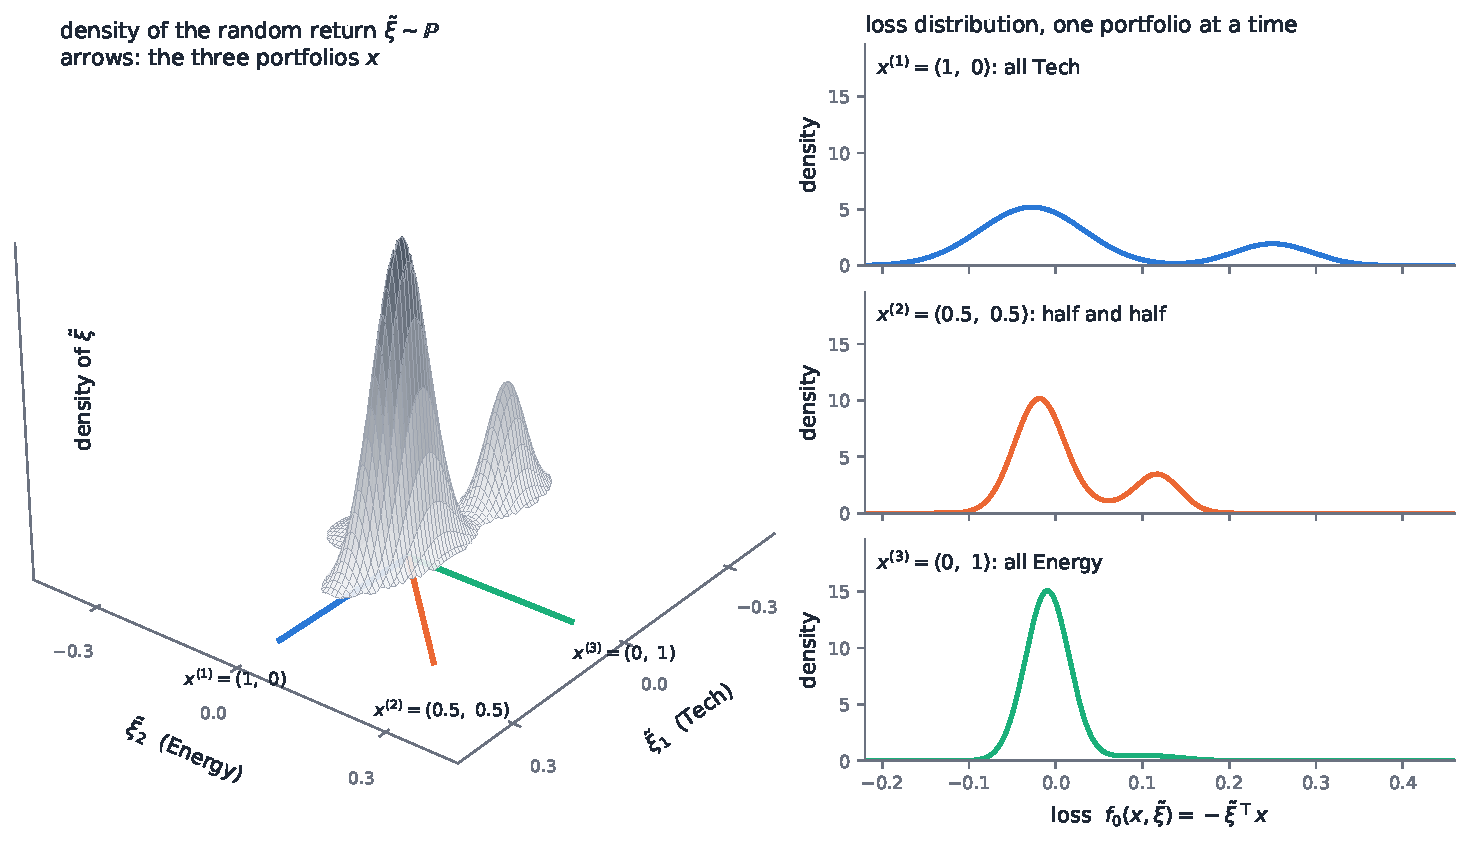
\includegraphics[width=0.78\textwidth]{week09_loss_distribution.pdf}
\end{center}
\vspace{0pt}

\quad how do we compare the three? \ we need one number per distribution: \ the risk measure $\R_{\Prob}$.
\vspace{8pt}

\end{board}

\subbeat{2.1}{Risk neutral}
\begin{board}
$\R_{\Prob} = \E_{\Prob}$ \ : \ expected value
\vspace{6pt}

\quad \textbf{minimizing $\E_{\Prob}$ over $x$:}
\vspace{2pt}

\begin{center}
$\displaystyle \min_{x \in \mathcal{X}}\ \E_{\Prob}\big[f_0(x, \xit)\big]$
\end{center}
\vspace{2pt}

\begin{center}
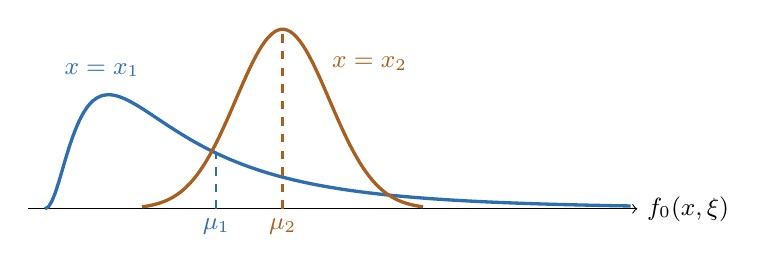
\begin{tikzpicture}[font=\small, x=0.85cm, y=0.8cm]
  % lognormal(0.64, 0.8^2) vs normal(3.6, 0.7^2), same scale; means 2.61 and 3.60, by integration and simulation
  \draw[->] (-0.2,0) -- (8.9,0) node[right] {$f_0(x, \xi)$};
  \draw[very thick, lineA, domain=0.05:8.8, samples=170] plot (\x, {5*exp(-(ln(\x)-0.64)^2/1.28)/(\x*0.8*2.5066)});
  \draw[very thick, lineB, domain=1.5:5.7, samples=90] plot (\x, {2.85*exp(-(\x-3.6)^2/0.98)});
  \draw[dashed, thick, lineA] (2.61,0) -- (2.61,0.88);
  \draw[dashed, thick, lineB] (3.60,0) -- (3.60,2.85);
  \node[below, lineA] at (2.61,0) {$\mu_1$};
  \node[below, lineB] at (3.60,0) {$\mu_2$};
  \node[lineA] at (0.9,2.2) {$x = x_1$};
  \node[lineB] at (4.9,2.3) {$x = x_2$};
\end{tikzpicture}
\end{center}
\vspace{2pt}

\quad $\mu_1 = \E_{\Prob}[f_0(x_1, \xit)] \;<\; \mu_2 = \E_{\Prob}[f_0(x_2, \xit)]$
\quad $\Rightarrow$ \ $x_1$ is preferable under the risk-neutral measure.
\end{board}

\newpage

% ---------------------------------------------------------------- 2.2
\subbeat{2.2}{Risk averse 1: mean--variance}
\begin{board}
$\R_{\Prob} = \lambda\,\mathrm{Var}_{\Prob} + (1-\lambda)\,\E_{\Prob}$ \ : \ convex combination of mean and variance
\vspace{6pt}

\quad \textbf{minimizing mean--variance over $x$:}
\vspace{2pt}

\begin{center}
$\displaystyle \min_{x \in \mathcal{X}}\ \ \lambda\,\mathrm{Var}_{\Prob}\big[f_0(x, \xit)\big] + (1 - \lambda)\,\E_{\Prob}\big[f_0(x, \xit)\big]$
\qquad $\lambda \in [0, 1]$
\end{center}
\vspace{8pt}

\textbf{Example (Mean--variance portfolio optimization)} \quad (Harry Markowitz, 1952)
\vspace{2pt}

\quad $\xit \in \mathbb{R}^n$ is the vector of asset returns. \quad Assume we know
\vspace{3pt}

\qquad $\E_{\Prob}[\xit] = \mu$ \quad vector of means, \qquad
$\E_{\Prob}\big[(\xit - \mu)(\xit - \mu)^{\top}\big] = \E_{\Prob}[\xit\xit^{\top}] - \mu\mu^{\top} = \Sigma$ \quad covariance matrix
\vspace{6pt}

\quad an investor allocates a wealth of $\$1$ to minimize the mean--variance of the portfolio loss $-\xit^{\top}x$:
\vspace{4pt}

\begin{center}
\fbox{\rule{0pt}{1em}\;
$\begin{aligned}
  \min\quad & \lambda\,\mathrm{Var}_{\Prob}\big(-\xit^{\top}x\big) + (1-\lambda)\,\E_{\Prob}\big[-\xit^{\top}x\big] \\
  \text{s.t.}\quad & e^{\top}x = 1 \\
                   & x \ge 0
\end{aligned}$
\;\rule[-2.6em]{0pt}{1em}}
\end{center}
\vspace{8pt}

\begin{center}
\fbox{\parbox{0.96\linewidth}{%
(Review: HW\#2) \ \textbf{reformulate} --- both terms are functions of $\mu$ and $\Sigma$ only:
\vspace{4pt}

\quad $\E_{\Prob}[-\xit^{\top}x] = -\mu^{\top}x$ \qquad linearity of expectation
\vspace{6pt}

\quad $\begin{aligned}[t]
  \mathrm{Var}_{\Prob}(-\xit^{\top}x) = \mathrm{Var}_{\Prob}(\xit^{\top}x)
    &= \E_{\Prob}\big[(\xit^{\top}x)^2\big] - \big(\E_{\Prob}[\xit^{\top}x]\big)^2 \\
    &= \E_{\Prob}\big[x^{\top}\xit\xit^{\top}x\big] - (\mu^{\top}x)^2
     = x^{\top}\E_{\Prob}[\xit\xit^{\top}]\,x - x^{\top}\mu\mu^{\top}x \\
    &= x^{\top}\big(\E_{\Prob}[\xit\xit^{\top}] - \mu\mu^{\top}\big)x \\
    &= x^{\top}\Sigma\,x
\end{aligned}$
\vspace{8pt}

\begin{center}
$\begin{aligned}
  \min\quad & \lambda\,x^{\top}\Sigma\,x - (1-\lambda)\,\mu^{\top}x \\
  \text{s.t.}\quad & e^{\top}x = 1 \\
                   & x \ge 0
\end{aligned}$
\qquad $\Sigma \succeq 0$ \ $\Rightarrow$ \ convex quadratic program
\end{center}
}}
\end{center}
\vspace{6pt}

\textbf{Limits of mean--variance}
\vspace{4pt}

\bul for a general loss $f_0(x, \xit)$, \ $\mathrm{Var}_{\Prob}[f_0(x, \xit)]$ need not be convex in $x$ \ --- the mean--variance
risk measure in general leads to a non-convex optimization problem. \ (the above model is an exception: \ $f_0(x, \xi) = -\xi^{\top}x$ is linear, hence the variance term leads to a quadratic function, hence convex)
\vspace{6pt}

\bul variance penalizes spread in \emph{both} directions --- it does not see where the big losses are:
\vspace{4pt}

\begin{center}
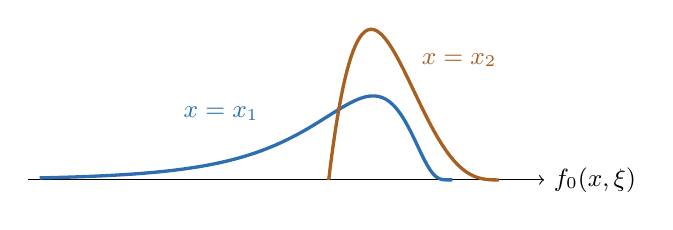
\begin{tikzpicture}[font=\small, x=0.72cm, y=0.8cm]
  % x1 = 4.3 - lognormal(0.708, 0.6^2): Var 2.55, long left side, short right side
  % x2 = 2.1 + 3 Beta(2,4) on [2.1, 5.1]: Var 0.29; both densities integrate to 1 and share the scale 3.4
  % P(x2 > t) >= P(x1 > t) at every level t
  \draw[->] (-3.2,0) -- (5.9,0) node[right] {$f_0(x, \xi)$};
  \draw[very thick, lineA, domain=-3.0:4.28, samples=150] plot (\x, {3.4*exp(-(ln(4.3-\x)-0.708)^2/0.72)/((4.3-\x)*0.6*2.5066)});
  \draw[very thick, lineB, domain=2.1:5.1, samples=120] plot (\x, {3.4*(20/3)*((\x-2.1)/3)*(1-(\x-2.1)/3)^3});
  \node[lineA] at (0.2,1.05) {$x = x_1$};
  \node[lineB] at (4.4,1.9) {$x = x_2$};
\end{tikzpicture}
\end{center}
\vspace{-2pt}

\qquad $x_2$ has lower variance, but has higher probability of generating bigger losses.
\vspace{4pt}

\begin{center}
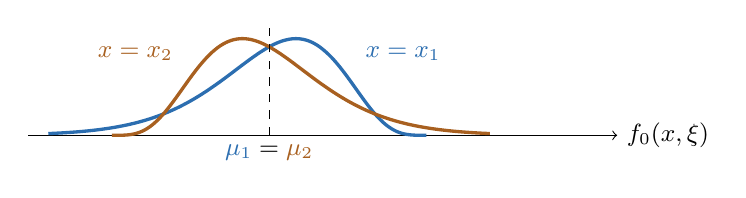
\begin{tikzpicture}[font=\small, x=0.85cm, y=0.8cm]
  % mirror images about the mean 3.4: same mean, same variance.  Gamma(k=6, theta=0.4) shape, unimodal,
  % mildly skewed; x2 = 1.0 + Gamma (tail toward large losses), x1 = 5.8 - Gamma (tail toward small losses)
  \draw[->] (-0.2,0) -- (8.6,0) node[right] {$f_0(x, \xi)$};
  \draw[very thick, lineA, domain=0.1:5.75, samples=140] plot (\x, {0.0729*exp(5*ln((5.8-\x)/0.4) - (5.8-\x)/0.4)});
  \draw[very thick, lineB, domain=1.05:6.7, samples=140] plot (\x, {0.0729*exp(5*ln((\x-1.0)/0.4) - (\x-1.0)/0.4)});
  \draw[dashed] (3.4,0) -- (3.4,1.7);
  \node[below] at (3.4,0) {${\color{lineA}\mu_1} = {\color{lineB}\mu_2}$};
  \node[lineA] at (5.4,1.3) {$x = x_1$};
  \node[lineB] at (1.4,1.3) {$x = x_2$};
\end{tikzpicture}
\end{center}
\vspace{-2pt}

\qquad $x_1$ and $x_2$ have the same mean and the same variance (mirror images), so mean--variance cannot tell
them apart; \ but $x_1$ is preferred because it has higher probability of generating smaller losses.
\end{board}

\newpage

% ---------------------------------------------------------------- 2.3
\subbeat{2.3}{Risk averse 2: Value at Risk (VaR)}
\begin{board}
$\R_{\Prob} = \VaR_{\varepsilon}$ \ : \ $(1 - \varepsilon)$-quantile of the loss
\quad typically a non-convex optimization problem
\vspace{3pt}

\quad {\small Of course, $\VaR_{\varepsilon}$ depends on $\Prob$ just like $\E_{\Prob}$ and $\mathrm{Var}_{\Prob}$; \ we omit the index for notational simplicity.}
\vspace{6pt}

\begin{center}
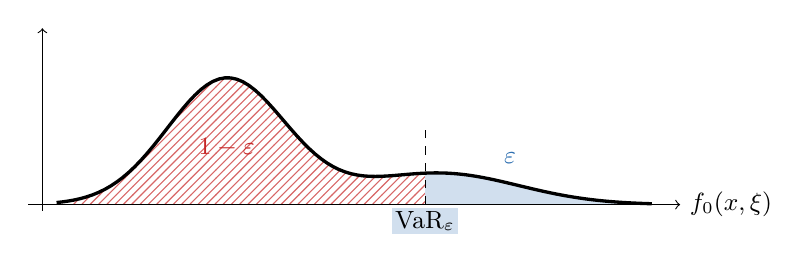
\begin{tikzpicture}[font=\small, x=0.9cm, y=0.8cm]
  % density g = 2.0 N-bump(2.6, 1.4) + 0.5 N-bump(5.6, 2.5);  VaR at 5.4 cuts off eps = 0.14 of the mass
  \fill[pattern=north east lines, pattern color=redink!70]
    (0.4,0) -- plot[domain=0.4:5.4, samples=70] (\x, {2.0*exp(-(\x-2.6)^2/1.4) + 0.5*exp(-(\x-5.6)^2/2.5)}) -- (5.4,0) -- cycle;
  \fill[lineA!22]
    (5.4,0) -- plot[domain=5.4:8.6, samples=60] (\x, {2.0*exp(-(\x-2.6)^2/1.4) + 0.5*exp(-(\x-5.6)^2/2.5)}) -- (8.6,0) -- cycle;
  \draw[->] (-0.2,0) -- (9.0,0) node[right] {$f_0(x, \xi)$};
  \draw[->] (0,-0.1) -- (0,2.8);
  \draw[very thick, black, domain=0.2:8.6, samples=100] plot (\x, {2.0*exp(-(\x-2.6)^2/1.4) + 0.5*exp(-(\x-5.6)^2/2.5)});
  \node[redink] at (2.6,0.9) {$1 - \varepsilon$};
  \draw[dashed] (5.4,0) -- (5.4,1.2);
  \node[lineA, above] at (6.6,0.5) {$\varepsilon$};
  \node[below, fill=lineA!22, inner sep=1pt] at (5.4,-0.05) {$\VaR_{\varepsilon}$};
\end{tikzpicture}
\end{center}
\vspace{2pt}

\quad --- popular in finance
\vspace{2pt}

\quad --- imposed by the Basel II accord: how much capital banks need to set aside to hold against financial risks
\vspace{12pt}

\textbf{Formally:}
\vspace{2pt}

\begin{center}
\fbox{\rule{0pt}{1em}\;
$\begin{aligned}
  \VaR_{\varepsilon}\big[f_0(x, \xit)\big] \;=\; \min_{t \in \mathbb{R}}\ \ & t \\
  \text{s.t.}\ \ & \Prob\big(f_0(x, \xit) \le t\big) \ge 1 - \varepsilon
\end{aligned}$
\;\rule[-1.4em]{0pt}{1em}}
\end{center}
\vspace{4pt}

\quad the constraint is a chance / probability constraint: \ generally non-convex, highly intractable
\vspace{3pt}

\quad the smallest loss level $t$ that is exceeded with probability at most $\varepsilon$
\vspace{6pt}

\begin{minipage}{\dimexpr\linewidth-1.3em\relax}
\quad \textbf{minimizing VaR over $x$:} \ the $\min$ over $t$ joins the outer $\min$ over $x$
\vspace{2pt}

\begin{center}
$\begin{aligned}
  \min_{x \in \mathcal{X}}\ \VaR_{\varepsilon}\big[f_0(x, \xit)\big]
  &= \min_{x \in \mathcal{X}}\ \min_{t \in \mathbb{R}}\ \ t \quad \text{s.t.} \quad \Prob\big(f_0(x, \xit) \le t\big) \ge 1 - \varepsilon \\
  &= \min_{x \in \mathcal{X},\ t \in \mathbb{R}}\ \ t \quad \text{s.t.} \quad \Prob\big(f_0(x, \xit) \le t\big) \ge 1 - \varepsilon
\end{aligned}$
\end{center}
\end{minipage}
\vspace{4pt}

\quad VaR risk measure in general leads to a non-convex optimization problem.
\end{board}

% ---------------------------------------------------------------- 2.4
\subbeat{2.4}{Risk averse 3: Conditional Value at Risk (CVaR)}
\begin{board}
$\R_{\Prob} = \CVaR_{\varepsilon}$ \ : \ average loss in the worst $\varepsilon$ fraction of outcomes
\quad convex if $f_0$ is convex in $x$
\vspace{6pt}

\begin{center}
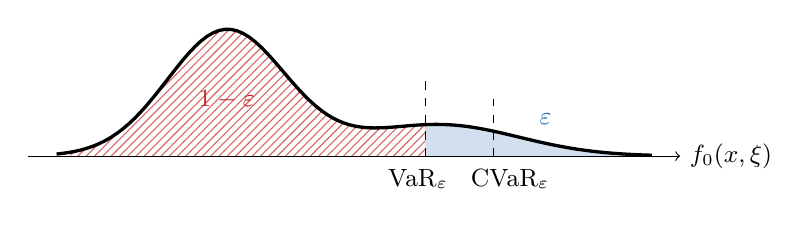
\begin{tikzpicture}[font=\small, x=0.9cm, y=0.8cm]
  % same density and VaR as the VaR picture;  CVaR = conditional mean of the tail beyond VaR = 6.37
  \fill[pattern=north east lines, pattern color=redink!70]
    (0.4,0) -- plot[domain=0.4:5.4, samples=70] (\x, {2.0*exp(-(\x-2.6)^2/1.4) + 0.5*exp(-(\x-5.6)^2/2.5)}) -- (5.4,0) -- cycle;
  \fill[lineA!22]
    (5.4,0) -- plot[domain=5.4:8.6, samples=60] (\x, {2.0*exp(-(\x-2.6)^2/1.4) + 0.5*exp(-(\x-5.6)^2/2.5)}) -- (8.6,0) -- cycle;
  \draw[->] (-0.2,0) -- (9.0,0) node[right] {$f_0(x, \xi)$};
  \draw[very thick, black, domain=0.2:8.6, samples=100] plot (\x, {2.0*exp(-(\x-2.6)^2/1.4) + 0.5*exp(-(\x-5.6)^2/2.5)});
  \node[redink] at (2.6,0.9) {$1 - \varepsilon$};
  \draw[dashed] (5.4,0) -- (5.4,1.2);
  \draw[dashed] (6.37,0) -- (6.37,0.9);
  \node[lineA, above] at (7.1,0.35) {$\varepsilon$};
  \node[below] at (5.3,-0.05) {$\VaR_{\varepsilon}$};
  \node[below] at (6.6,-0.05) {$\CVaR_{\varepsilon}$};
\end{tikzpicture}
\end{center}
\vspace{2pt}

\begin{minipage}{\dimexpr\linewidth-1.3em\relax}
\quad with $\Zt = f_0(x, \xit)$: \ CVaR is the average loss in the tail beyond $\VaR_{\varepsilon}$, \ i.e., a conditional expectation:
\vspace{4pt}

\textbf{Def (conditional expectation)} \qquad
$\displaystyle \E_{\Prob}\big[\Zt \,\big|\, \Zt \in A\big] = \frac{\E_{\Prob}\big[\Zt\,\ind{\Zt \in A}\big]}{\Prob(\Zt \in A)}$
\vspace{2pt}

\begin{center}
\fbox{\rule{0pt}{1em}\;
\textbf{Proposition:} \ if $\Zt$ has a continuous distribution, then \quad
$\CVaR_{\varepsilon}[\Zt] = \E_{\Prob}\big[\Zt \,\big|\, \Zt \ge \VaR_{\varepsilon}[\Zt]\big]$
\;\rule[-0.6em]{0pt}{1em}}
\end{center}
\vspace{2pt}

\quad here $A$ is the tail, of probability $\varepsilon$: \qquad
$\displaystyle \CVaR_{\varepsilon}[\Zt] = \frac{1}{\varepsilon}\,\E_{\Prob}\big[\Zt\,\ind{\Zt \ge \VaR_{\varepsilon}[\Zt]}\big]$
\end{minipage}
\vspace{4pt}

\quad --- CVaR = the \textbf{average loss in the worst $\varepsilon$ fraction} of outcomes; \ so \ $\CVaR_{\varepsilon} \ge \VaR_{\varepsilon}$.
\vspace{2pt}

\quad --- introduced by Rockafellar \& Uryasev (2000)
\vspace{2pt}

\quad --- imposed by the Basel III accord
\vspace{12pt}

\begin{minipage}{\dimexpr\linewidth-1.3em\relax}
\textbf{Formally:}
\vspace{2pt}

\begin{center}
\fbox{\rule{0pt}{1em}\;
$\displaystyle \CVaR_{\varepsilon}\big[f_0(x, \xit)\big] \;=\; \min_{\beta \in \mathbb{R}}\ \
  \beta + \frac{1}{\varepsilon}\,\E_{\Prob}\Big[\max\big\{f_0(x, \xit) - \beta,\ 0\big\}\Big]$
\;\rule[-1.4em]{0pt}{1em}}
\end{center}
\end{minipage}
\vspace{4pt}

\quad this formula works for \emph{any} distribution of $\Zt$; \ for a continuous $\Zt$ it equals the conditional expectation above
\vspace{4pt}

\begin{minipage}{\dimexpr\linewidth-1.3em\relax}
\quad \textbf{minimizing CVaR over $x$:} \ the $\min$ over $\beta$ joins the outer $\min$ over $x$
\vspace{2pt}

\begin{center}
$\begin{aligned}
  \min_{x \in \mathcal{X}}\ \CVaR_{\varepsilon}\big[f_0(x, \xit)\big]
  &= \min_{x \in \mathcal{X}}\ \min_{\beta \in \mathbb{R}}\ \ \beta + \frac{1}{\varepsilon}\,\E_{\Prob}\Big[\max\big\{f_0(x, \xit) - \beta,\ 0\big\}\Big] \\
  &= \min_{x \in \mathcal{X},\ \beta \in \mathbb{R}}\ \ \beta + \frac{1}{\varepsilon}\,\E_{\Prob}\Big[\max\big\{f_0(x, \xit) - \beta,\ 0\big\}\Big]
\end{aligned}$
\end{center}
\end{minipage}
\vspace{4pt}

\quad the objective is convex in $(x, \beta)$ when $f_0$ is convex in $x$: \ $\max\{\text{convex}, 0\}$ is convex,
and $\E$ keeps it convex.
\vspace{6pt}

\begin{minipage}{\dimexpr\linewidth-1.3em\relax}
\quad \textbf{why CVaR is convex:} \ build it from convex pieces, \ with the operations from HW1 and week 2
\vspace{2pt}

\begin{center}
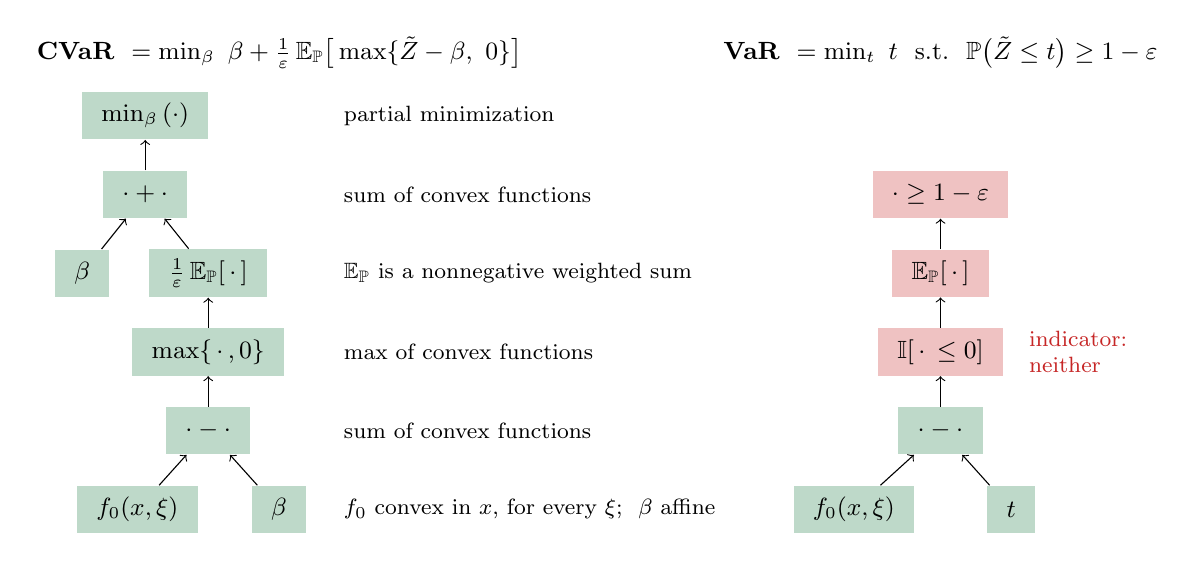
\begin{tikzpicture}[font=\small,
  op/.style={rectangle, minimum height=0.6cm, inner xsep=7pt},
  good/.style={op, fill=grnink!28},
  bad/.style={op, fill=redink!28},
  why/.style={anchor=west, font=\footnotesize}]
  \def\h{1.0}
  % CVaR
  \node[anchor=west] at (-0.2,5.8) {\textbf{CVaR} \ $= \min_{\beta}\ \beta + \tfrac{1}{\varepsilon}\,\E_{\Prob}\big[\max\{\Zt - \beta,\ 0\}\big]$};
  \node[good] (cf) at (1.2,0*\h) {$f_0(x, \xi)$};
  \node[good] (cb) at (3.0,0*\h) {$\beta$};
  \node[good] (c1) at (2.1,1*\h) {$\cdot - \cdot$};
  \node[good] (c2) at (2.1,2*\h) {$\max\{\,\cdot\,, 0\}$};
  \node[good] (c3) at (2.1,3*\h) {$\frac{1}{\varepsilon}\,\E_{\Prob}[\,\cdot\,]$};
  \node[good] (b2) at (0.5,3*\h) {$\beta$};
  \node[good] (c4) at (1.3,4*\h) {$\cdot + \cdot$};
  \node[good] (c5) at (1.3,5*\h) {$\min_{\beta}\,(\cdot)$};
  \foreach \a/\b in {cf/c1, cb/c1, c1/c2, c2/c3, c3/c4, b2/c4, c4/c5} \draw[->] (\a) -- (\b);
  % why each CVaR step is convex
  \node[why] at (3.7,0*\h) {$f_0$ convex in $x$, for every $\xi$; \ $\beta$ affine};
  \node[why] at (3.7,1*\h) {sum of convex functions};
  \node[why] at (3.7,2*\h) {max of convex functions};
  \node[why] at (3.7,3*\h) {$\E_{\Prob}$ is a nonnegative weighted sum};
  \node[why] at (3.7,4*\h) {sum of convex functions};
  \node[why] at (3.7,5*\h) {partial minimization};
  % VaR: the chance constraint, P(Z <= t) = E[indicator] >= 1 - eps
  \node at (11.4,5.8) {\textbf{VaR} \ $= \min_{t}\ t \ \ \text{s.t.}\ \ \Prob\big(\Zt \le t\big) \ge 1 - \varepsilon$};
  \node[good] (vf) at (10.3,0*\h) {$f_0(x, \xi)$};
  \node[good] (vt) at (12.3,0*\h) {$t$};
  \node[good] (v1) at (11.4,1*\h) {$\cdot - \cdot$};
  \node[bad]  (v2) at (11.4,2*\h) {$\ind{\,\cdot\, \le 0}$};
  \node[bad]  (v3) at (11.4,3*\h) {$\E_{\Prob}[\,\cdot\,]$};
  \node[bad]  (v4) at (11.4,4*\h) {$\cdot \ge 1 - \varepsilon$};
  \foreach \a/\b in {vf/v1, vt/v1, v1/v2, v2/v3, v3/v4} \draw[->] (\a) -- (\b);
  \node[anchor=west, font=\footnotesize, redink, align=left] at (12.4,2*\h) {indicator:\\neither};
\end{tikzpicture}
\end{center}
\vspace{-4pt}

\quad {\footnotesize green: convex or affine, jointly in $(x, \beta)$ or $(x, t)$ \quad\textbullet\quad red: neither}
\end{minipage}
\vspace{4pt}

\quad for VaR, the chance constraint leads to the indicator, \ $\Prob(\Zt \le t) = \E_{\Prob}\big[\ind{\Zt \le t}\big] \ge 1 - \varepsilon$, \ i.e., a MIP.
\vspace{3pt}

\quad here $\E_{\Prob}\big[\ind{A}\big] = 1 \cdot \Prob(A) + 0 \cdot \big(1 - \Prob(A)\big) = \Prob(A)$, \ since $\ind{A}$ is $1$ exactly when $A$ holds
\vspace{10pt}

\textbf{Proof of the Proposition:} \quad step 1 --- find the minimizer $\beta^{*}$.
\vspace{3pt}

\quad $\displaystyle \frac{\partial}{\partial\beta}\Big(\beta + \frac{1}{\varepsilon}\,\E_{\Prob}\big[\max\{\Zt - \beta, 0\}\big]\Big) = 0$
\vspace{3pt}

\quad $\displaystyle 1 + \frac{1}{\varepsilon}\,\E_{\Prob}\Big[\frac{\partial}{\partial\beta}\max\{\Zt - \beta, 0\}\Big] = 0$
\hspace{1.5cm}
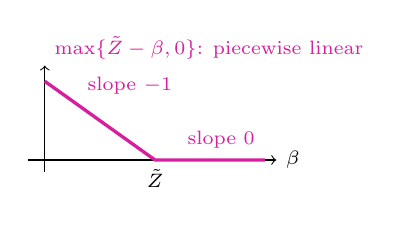
\begin{tikzpicture}[baseline=0.4cm, font=\scriptsize, x=0.7cm, y=0.5cm]
  \draw[->] (-0.3,0) -- (4.2,0) node[right] {$\beta$};
  \draw[->] (0,-0.3) -- (0,2.4);
  \draw[very thick, magink] (0,2.0) -- (2.0,0) -- (4.0,0);
  \node[below] at (2.0,0) {$\Zt$};
  \node[magink, right] at (0.6,1.9) {slope $-1$};
  \node[magink, above] at (3.2,0.05) {slope $0$};
  \node[magink, above right] at (0,2.3) {$\max\{\Zt - \beta, 0\}$: piecewise linear};
\end{tikzpicture}
\vspace{3pt}

\quad $\displaystyle 1 + \frac{1}{\varepsilon}\,\E_{\Prob}\big[-\ind{\Zt > \beta}\big] = 0$
\hspace{2.2cm}indicator function: \ $\ind{A} = \begin{cases} 1 & \text{if } A \text{ holds} \\ 0 & \text{otherwise}\end{cases}$
\vspace{3pt}

\quad $\displaystyle 1 - \frac{1}{\varepsilon}\,\Prob(\Zt > \beta) = 0$
\hspace{3.3cm}$\E_{\Prob}[\ind{A}] = \Prob(A)$
\vspace{3pt}

\quad $\Prob(\Zt > \beta) = \varepsilon$ \qquad $\Rightarrow$ \qquad $\beta^{*} = \VaR_{\varepsilon}[\Zt]$
\vspace{5pt}

\begin{minipage}{\dimexpr\linewidth-1.3em\relax}
\quad step 2 --- plug $\beta^{*}$ in. \quad Since $\Zt$ is continuous, \ $\Prob(\Zt \ge \beta^{*}) = \Prob(\Zt > \beta^{*}) = \varepsilon$:
\vspace{3pt}

\quad $\begin{aligned}[t]
  \CVaR_{\varepsilon}[\Zt]
    &= \beta^{*} + \frac{1}{\varepsilon}\,\E_{\Prob}\big[\max\{\Zt - \beta^{*}, 0\}\big] \\
    &= \beta^{*} + \frac{1}{\varepsilon}\,\E_{\Prob}\big[(\Zt - \beta^{*})\,\ind{\Zt \ge \beta^{*}}\big] \\
    &= \beta^{*} + \frac{1}{\Prob(\Zt \ge \beta^{*})}\,\E_{\Prob}\big[\Zt\,\ind{\Zt \ge \beta^{*}}\big]
       - \frac{1}{\Prob(\Zt \ge \beta^{*})}\,\E_{\Prob}\big[\beta^{*}\,\ind{\Zt \ge \beta^{*}}\big] \\
    &= \beta^{*} + \E_{\Prob}\big[\Zt \,\big|\, \Zt \ge \beta^{*}\big] - \beta^{*} \\
    &= \E_{\Prob}\big[\Zt \,\big|\, \Zt \ge \VaR_{\varepsilon}[\Zt]\big] \qquad \blacksquare
\end{aligned}$
\end{minipage}
\end{board}

\begin{board}
\textbf{$\Zt$ has a discrete distribution} --- what does the proposition become?
\vspace{4pt}

\quad Consider: \ $\Prob(\Zt = 1) = \tfrac14$, \quad $\Prob(\Zt = 0) = \tfrac12$, \quad $\Prob(\Zt = -1) = \tfrac14$.
\qquad Let \ $\varepsilon = \tfrac12$.
\hspace{1.0cm}
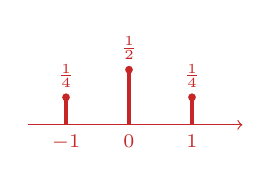
\begin{tikzpicture}[baseline=0.1cm, font=\scriptsize, x=0.8cm, y=1.4cm]
  \draw[->, redink] (-1.6,0) -- (1.8,0);
  \foreach \p/\h in {-1/0.25, 0/0.5, 1/0.25} {
    \draw[very thick, redink] (\p,0) -- (\p,\h);
    \fill[redink] (\p,\h) circle (1.4pt);
    \node[below, redink] at (\p,0) {$\p$};
  }
  \node[redink, above] at (-1,0.25) {$\tfrac14$};
  \node[redink, above] at (0,0.5) {$\tfrac12$};
  \node[redink, above] at (1,0.25) {$\tfrac14$};
\end{tikzpicture}
\vspace{4pt}

\quad $\begin{aligned}[t]
  \VaR_{\varepsilon}[\Zt] = \min_{t \in \mathbb{R}}\ \ & t \\
  \text{s.t.}\ \ & \Prob(\Zt \le t) \ge 1 - \tfrac12
\end{aligned}$
\quad $= 0$ \qquad {\small ($\Prob(\Zt \le 0) = \tfrac34 \ge \tfrac12$, \ and for any $t < 0$, \ $\Prob(\Zt \le t) \le \tfrac14$)}
\vspace{5pt}

\quad $\begin{aligned}[t]
  \CVaR_{\varepsilon}[\Zt]
    &= \min_{\beta \in \mathbb{R}}\ \beta + \frac{1}{\varepsilon}\,\E_{\Prob}\big[\max\{\Zt - \beta, 0\}\big] \\
    &= \min_{\beta \in \mathbb{R}}\ \beta + \frac{1}{1/2}\Big( \tfrac14 \max\{1 - \beta, 0\}
       + \tfrac12 \max\{0 - \beta, 0\} + \tfrac14 \max\{-1 - \beta, 0\} \Big) \\
    &= \tfrac12 \qquad {\small \text{(attained at } \beta = 0\text{: the objective is } \tfrac12 + \tfrac{\beta}{2} \text{ on } [0,1]
       \text{ and } \tfrac12 - \tfrac{\beta}{2} \text{ on } [-1, 0])}
\end{aligned}$
\vspace{5pt}

\quad but \quad $\displaystyle \E_{\Prob}\big[\Zt \,\big|\, \Zt \ge \underbrace{\VaR_{\varepsilon}[\Zt]}_{0}\big]
  = \frac{\tfrac12 \times 0 + \tfrac14 \times 1}{\tfrac12 + \tfrac14} = \tfrac13$
\qquad and \qquad
$\displaystyle \E_{\Prob}\big[\Zt \,\big|\, \Zt > \VaR_{\varepsilon}[\Zt]\big] = \frac{\tfrac14 \times 1}{\tfrac14} = 1$
\vspace{4pt}

\quad neither is $\tfrac12$: \ the atom at $\VaR_{\varepsilon}$ is too big --- $\Prob(\Zt \ge 0) = \tfrac34 > \varepsilon$ but $\Prob(\Zt > 0) = \tfrac14 < \varepsilon$.
\vspace{5pt}

\begin{minipage}{\dimexpr\linewidth-1.3em\relax}
\textbf{Atom splitting} \quad split the atom at $0$ so that exactly $\varepsilon = \tfrac12$ of the mass lies in the tail:
\hspace{0.8cm}
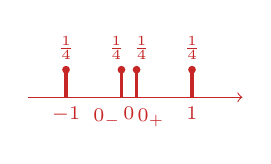
\begin{tikzpicture}[baseline=0.1cm, font=\scriptsize, x=0.8cm, y=1.4cm]
  \draw[->, redink] (-1.6,0) -- (1.8,0);
  \foreach \p/\h in {-1/0.25, -0.12/0.25, 0.12/0.25, 1/0.25} {
    \draw[very thick, redink] (\p,0) -- (\p,\h);
    \fill[redink] (\p,\h) circle (1.4pt);
  }
  \node[below, redink] at (-1,0) {$-1$}; \node[below, redink] at (0,0) {$0$}; \node[below, redink] at (1,0) {$1$};
  \node[redink, above] at (-1,0.25) {$\tfrac14$}; \node[redink, above] at (-0.2,0.25) {$\tfrac14$};
  \node[redink, above] at (0.2,0.25) {$\tfrac14$}; \node[redink, above] at (1,0.25) {$\tfrac14$};
  \node[redink, below] at (-0.35,-0.02) {$0_-$}; \node[redink, below] at (0.35,-0.02) {$0_+$};
\end{tikzpicture}
\vspace{4pt}

\quad $\displaystyle \E_{\Prob}\big[\Zt \,\big|\, \Zt \ge 0_+\big] = \frac{\tfrac14 \times 0 + \tfrac14 \times 1}{\tfrac12} = \tfrac12$
\qquad $= \CVaR_{\varepsilon}[\Zt]$ \quad $\checkmark$
\end{minipage}
\vspace{4pt}

\quad in general: CVaR = the average of the worst $\varepsilon$ of the probability mass, with the atom at $\VaR_{\varepsilon}$ split
as needed. \ The $\min_{\beta}$ formula gets this right automatically.
\end{board}

\newpage

% ---------------------------------------------------------------- 3
\beat{3}{Uncertainty in the constraint}
\begin{board}
Now uncertainty only in the constraints; \ the objective $f_0(x)$ is deterministic:
\vspace{2pt}

\begin{center}
$\displaystyle \min_{x \in \mathcal{X}}\ f_0(x)$ \quad s.t. \quad ${\color{redink}\R_{\Prob}\big[}f_i(x, \xit){\color{redink}\big]} \le 0 \quad \forall i \in [I]$
\end{center}
\vspace{2pt}

\vspace{2pt}

Three choices of $\R_{\Prob}$:
\vspace{4pt}

\quad --- $\E_{\Prob}\big[f_i(x, \xit)\big] \le 0$ \qquad\qquad the constraint holds \emph{on average}
\vspace{3pt}

\quad --- $\VaR_{\varepsilon}\big[f_i(x, \xit)\big] \le 0$
\qquad non-convex in general
\vspace{3pt}

\qquad $\displaystyle \iff\ \min_{t \in \mathbb{R}}\big\{\, t \;:\; \Prob\big(f_i(x, \xit) \le t\big) \ge 1 - \varepsilon \,\big\} \le 0$
\vspace{3pt}

\qquad $\displaystyle \iff\ \exists\, t \le 0 \;:\; \Prob\big(f_i(x, \xit) \le t\big) \ge 1 - \varepsilon$
\vspace{3pt}

\qquad $\displaystyle \iff\ \Prob\big(f_i(x, \xit) \le 0\big) \ge 1 - \varepsilon$
\vspace{3pt}

\textbf{Chance constraint / probabilistic constraint} \qquad
$\Prob\big(f_i(x, \xit) \le 0\big) \ge 1 - \varepsilon$
\vspace{5pt}

\begin{center}
\fbox{\rule{0pt}{1em}\;
\textbf{Proposition:} \quad $\VaR_{\varepsilon}$ constraint \ $\iff$ \ chance constraint
\;\rule[-0.6em]{0pt}{1em}}
\end{center}
\vspace{4pt}

\quad the chance constraint from week 10 is a VaR constraint: \ ``violated with probability at most $\varepsilon$''
\ is the same as \ ``the $(1-\varepsilon)$-quantile of $f_i$ is at most 0''.
\vspace{6pt}

\begin{minipage}{\dimexpr\linewidth-1.3em\relax}
\quad \textbf{the full problem:}
\vspace{2pt}

\begin{center}
\mbox{$\begin{array}{rl}
  \displaystyle\min_{x \in \mathcal{X}} & f_0(x) \\[6pt]
  \text{s.t.} & \VaR_{\varepsilon}\big[f_i(x, \xit)\big] \le 0 \quad \forall i \in [I]
\end{array}
\quad\iff\quad
\begin{array}{rl}
  \displaystyle\min_{x \in \mathcal{X}} & f_0(x) \\[6pt]
  \text{s.t.} & \Prob\big(f_i(x, \xit) \le 0\big) \ge 1 - \varepsilon \quad \forall i \in [I]
\end{array}$}
\end{center}
\end{minipage}
\vspace{6pt}

\quad --- $\CVaR_{\varepsilon}\big[f_i(x, \xit)\big] \le 0$
\qquad convex; gives an upper bound on $\VaR_{\varepsilon}$, so it implies the VaR constraint
\vspace{3pt}

\qquad $\displaystyle \iff\ \min_{\beta}\ \beta + \frac{1}{\varepsilon}\,\E_{\Prob}\big[\max\{f_i(x, \xit) - \beta, 0\}\big] \le 0$
\vspace{3pt}

\qquad $\displaystyle \iff\ \exists\, \beta \in \mathbb{R} \;:\; \beta + \frac{1}{\varepsilon}\,\E_{\Prob}\big[\max\{f_i(x, \xit) - \beta, 0\}\big] \le 0$
\vspace{6pt}

\begin{minipage}{\dimexpr\linewidth-1.3em\relax}
\quad \textbf{the full problem} \ --- \ the $\exists\, \beta$ becomes a decision variable, one $\beta_i$ per constraint
\vspace{2pt}

\begin{center}
\mbox{$\begin{array}{rl}
  \displaystyle\min_{x \in \mathcal{X}} & f_0(x) \\[6pt]
  \text{s.t.} & \CVaR_{\varepsilon}\big[f_i(x, \xit)\big] \le 0 \ \ \forall i \in [I]
\end{array}
\quad\iff\quad
\begin{array}{rl}
  \displaystyle\min_{x \in \mathcal{X},\ \beta \in \mathbb{R}^I} & f_0(x) \\[6pt]
  \text{s.t.} & \displaystyle \beta_i + \frac{1}{\varepsilon}\,\E_{\Prob}\big[\max\{f_i(x, \xit) - \beta_i, 0\}\big] \le 0 \ \ \forall i \in [I]
\end{array}$}
\end{center}
\end{minipage}
\vspace{10pt}

\begin{center}
\fbox{\rule{0pt}{1em}\;
\textbf{CVaR is a tractable conservative approximation of VaR, hence of the chance constraint}
\;\rule[-0.6em]{0pt}{1em}}
\end{center}
\vspace{2pt}

\quad for every $x$: \ $\VaR_{\varepsilon}[f_i] \le \CVaR_{\varepsilon}[f_i]$, \ since the average loss in the tail is at least where the tail starts
\vspace{3pt}

\quad so imposing \ $\CVaR_{\varepsilon}[f_i] \le 0$ \ forces \ $\VaR_{\varepsilon}[f_i] \le 0$, \ which is the chance constraint \ $\Prob(f_i \le 0) \ge 1 - \varepsilon$
\vspace{5pt}

\quad --- \textbf{tractable:} \ CVaR is convex when $f_i$ is convex in $x$; \ the chance constraint is NP-hard in general
\vspace{2pt}

\quad --- \textbf{conservative:} \ every $x$ feasible for CVaR is feasible for the chance constraint, \ but not vice versa
\end{board}

\newpage

% ---------------------------------------------------------------- 4
\beat{4}{Uncertainty in both: the CVaR stochastic program}
\begin{board}
\quad one $\beta$ per risk term: \ $\beta_0$ for the objective, $\beta_i$ for constraint $i$; \ all of them join the outer $\min$
\vspace{4pt}

\begin{center}
$\begin{aligned}
  \min_{x \in \mathcal{X},\ \beta_0, \dots, \beta_I \in \mathbb{R}}\quad
    & \beta_0 + \frac{1}{\varepsilon}\,\E_{\Prob}\Big[\max\big\{f_0(x, \xit) - \beta_0,\ 0\big\}\Big] \\
  \text{s.t.}\quad
    & \beta_i + \frac{1}{\varepsilon}\,\E_{\Prob}\Big[\max\big\{f_i(x, \xit) - \beta_i,\ 0\big\}\Big] \le 0 \qquad \forall i \in [I]
\end{aligned}$
\end{center}
\vspace{4pt}

\quad convex whenever every $f_i$ is convex in $x$.
\vspace{5pt}

\quad \textbf{with the discrete $\Prob$ from the recap}, \ replace each $\max$ by a variable $u_{is} \ge 0$
\vspace{4pt}

\begin{center}
$\begin{aligned}
  \min\quad & \beta_0 + \frac{1}{\varepsilon}\sum_{s \in [S]} p_s\, u_{0s} \\
  \text{s.t.}\quad & \beta_i + \frac{1}{\varepsilon}\sum_{s \in [S]} p_s\, u_{is} \le 0 && \forall i \in [I] \\
                   & u_{is} \ge f_i(x, \xi^s) - \beta_i, \quad u_{is} \ge 0 && \forall i \in \{0\} \cup [I],\ s \in [S] \\
                   & x \in \mathcal{X}
\end{aligned}$
\end{center}
\vspace{4pt}

\quad linear $f_i$ and polyhedral $\mathcal{X}$ \ $\Rightarrow$ \ a linear program, with no binary variables. \quad
The VaR / chance constraint needs a binary variable per scenario (which scenarios may violate the constraint)
--- the MIP in the recap. \ That is why CVaR is the tractable one.
\end{board}

\end{document}
